% Global
\documentclass[parskip=full,a4paper]{scrartcl}
\usepackage{blindtext}
\usepackage[utf8]{inputenc}
\usepackage{etoolbox}

% Graphics
\usepackage{pdfpages}
\usepackage{graphicx}

% Layout
% \usepackage{float}
\usepackage[margin=1in]{geometry}
\usepackage{setspace}
\setstretch{1.3}

% Inline-code
\usepackage[outputdir=./_build]{minted}
\setminted{fontsize=\scriptsize,baselinestretch=0}

% Bibliography
\usepackage{natbib}
\usepackage{bibentry}
\nobibliography*

% Title
\title{nETL}
\author{Zach Smith}
\date{\today}

 % Document
\begin{document}

\section{nETL}
Despite major disruptions to the University of Cape Town's teaching curriculum in 2016 xxx, the academic year was completed successfully with only minimal disruptions to the calendar schedule. Despite xxx hours of teaching time lost, xxx days of closing the university, course curriculums remained constant and exams tested a similar amount of material as had been previously tested.

One of the reasons the university could absorb such disruptions is due to their implementation of learning management software - their 'Vula' system, which is based on the 'Sukai' platform.

The trend of educational institutions has been to increasingly implement and rely on such software and UCT is no exception. Looking at a graph showing the uptake of such systems throughout globally acclaimed educational institutes shows just how important they have become xxx. A plethora of competing educational tools exist; Blackboard, Canvas, Sukai to name a few, all with a fairly comparable feature list xxx.

A key feature is ability to host and deliver course content via an online platform, taking advantage of functionality that such a platform can provide - in this case with reference to tracking of platform and content usage. With reference specifically to the Sakai platform, it is possible to follow which students accessed which resources and the timing of such events.

The striking at the University of Cape Town provides a unique opportunity to analyze this data as a comparison between classroom learning augmented by online tools vs primary reliance on online tools over an extended period by the same learners. Effectively a blind-control was inadvertently created that allows assessment of a single group of students in two isolated environments in terms of their resultant grades.

\section{cETL}
Many software packages exist to make analysis of such data trivial in terms of processing. Spreadsheet programs such as Microsoft Excel (or their online competition Google Sheets), databases such as Microsoft Access, MySQL are designed for this time of work.

But these tools fail when looking at scale of storage that Sakai's event data requires either in terms of ability (Microsoft Excel can work with a theoretical maximum of xxx lines, Access databases can be maximum 2GB), complexity or cost. Relational databases don't scale well horizontally speaking xxx, and this problem is going become more pronounced with time.

This thesis looks at creating a cost-effective 'analysis-engine' capable of scaling to many times the amount of data that a single machine can hold in a way that is still effective to analyze (distributed computing) and not too mentally taxing to implement.

specifically this project analyzed the viability of a software package called CouchDB, a NoSQL DBMS as a replacement for conventional RDMSs when analyzing data that has conventionally been housed RDBMSs (usually with an Oracle, Microsoft or SAP price tag associated with it).

% \newpage


\begin{figure}[H]
    \centering
    % \includegraphics[scale=0.4]{../resources/netlUML.pdf}
    \includepdf[pages={1},scale=0.7,pagecommand=\chapter]{../resources/figures/netlUML.pdf}
    \caption[nETL]{nETL}
    \label{nETL}
\end{figure}
\newpage

Coming from a relational database environment there are a plethora of tools avaialable that facilitate transfer of CSV dato to a DBMS. These tools are available at a variety of different levels of extraction depending on a users technical skillset, time constraints and requirements. xxx: list some of these tools.

In a SQL Server environment SSDT (formerly SSIS) is considered the de facto standard for extracting/transforming and loading data between different data sources. xxx: find a graph on the usage of SSDT/SSIS in companies.

In fact it's likely that the availability of of SSDT/SSIS has influenced the uptake of SQL Server in operations that require dealing with large amount of data. It's fair to say that a barrier to using open source software such as CouchDB is the LACK of such software. Bespoke scripts are currently the only viable way of interfacing with CouchDB in a way that is comparable to SQL Server and SSDT. But with high-level languages such as node.js maturing, and the proliferation of small, focused libraries in these languages that abstract much of the unpleasant and gnarly aspects of bespoke scripting (xxx examples), bespoke data-scripting is nowhere near as difficult as it would be within the Microsoft environment (C\# or VB).

In line with the requirement of transferring large amounts of CSV data from a CSV source to CouchDB, and taking into account the comparatively low entry barrier to bespoke data-transformation scripts, a component of this MSc is an exploration of a possible alternative to SSDT for an environment other than Microsoft's SQL Server. This MSc project actually has several requirements that fall within the ETL spectrum that such a framework could easily be adapted to handle in a generic way. The framework has been published as an npm library and is available at ..., with source code available at github somewhere xxx.

Fig. \ref{nETL} shows a potential architecture for a configurable component-based ETL tool...

such a framework that has been prototyped in node.js for this MSc.

% Appendix
\begin{appendix}
    \listoffigures
    \listoftables
\end{appendix}
\newpage

% Bibliogrpahy
\bibliographystyle{plain}
\bibliography{../bibliography/msc_citations.bib}

% Close docuemnt
\end{document}